\documentclass[
% draftcls,
% journal
]{IEEEtran}

\usepackage{graphicx}  % Include figure files
\usepackage{amsmath}   % Math symbols
\usepackage{cite}      % Citation formatting
\usepackage[table,xcdraw]{xcolor}  % Extended color definitions, including 'gray'
\usepackage{hyperref}  % Hyperlinks
\usepackage[caption=false,font=footnotesize]{subfig}  % Sub-figures
\usepackage{listings}  % Code listings

% Set code listing defaults
\lstset{
  basicstyle=\ttfamily\small,
  showstringspaces=false,
  language=c++,
  keywordstyle=\color{blue},
  commentstyle=\color{gray},
  breaklines=true
}

\begin{document}
\title{ASTE-404 Homework 7 Report}
\author{Luis~Diaz
\thanks{Student, Department of Astronautical Engineering, USC.}}
\markboth{ASTE-404 HW-7}{}
\maketitle
\IEEEpubid{\makebox[\columnwidth]{\copyright~2024 Luis Diaz} \hfill}

\begin{abstract}
This report demonstrates the integration of core software engineering practices, including code development, unit testing, documentation, version control, and report writing with \LaTeX. These processes collectively ensure robust, maintainable, and well-documented code \cite{particleincell}.
\end{abstract}

\begin{IEEEkeywords}
Google Test, Doxygen, GitHub, \LaTeX
\end{IEEEkeywords}

\section{Introduction}
This assignment aimed to implement software engineering principles across multiple stages. We focused on five key areas: code development, unit testing, documentation, version control, and report creation using \LaTeX. This report summarizes these practices, describing the tools and techniques applied.

References to online resources include various useful websites such as Slovak Cooking \cite{slovakcooking} and the personal blog of the project author \cite{iamlubos}. Additionally, the **Particle in Cell** journal article \cite{brieda2026} provides essential background on numerical simulations used in propulsion modeling.

\section{Part 1: Code Development}
Below is the C++ code defining a templated 3D vector class `vec3` with operations such as vector addition, subtraction, dot product, and magnitude calculation.

\begin{lstlisting}[caption={C++ Vector Code}, label={lst:code}]
#ifndef _VEC_H
#define _VEC_H
#include <ostream>
#include <math.h>

template<typename T>
class _vec3 {
public:
    _vec3<T>() : d{0, 0, 0} {}
    _vec3<T>(T a, T b, T c) : d{a, b, c} {}
    
    T& operator[] (int i) { return d[i]; }
    T operator[] (int i) const { return d[i]; }

    friend _vec3<T> operator+(const _vec3<T>& a, const _vec3<T>& b) {
        return _vec3<T>(a[0] + b[0], a[1] + b[1], a[2] + b[2]);
    }

    friend _vec3<T> operator-(const _vec3<T>& a, const _vec3<T>& b) {
        return _vec3<T>(a[0] - b[0], a[1] - b[1], a[2] - b[2]);
    }

    friend T dot(const _vec3<T>& a, const _vec3<T>& b) {
        return a[0] * b[0] + a[1] * b[1] + a[2] * b[2];
    }

    friend double mag(const _vec3<T>& a) {
        return sqrt(dot(a, a));
    }

    friend std::ostream& operator<<(std::ostream& out, const _vec3<T>& a) {
        out << a[0] << " " << a[1] << " " << a[2}; 
        return out;
    }

protected:
    T d[3];
};

using double3 = _vec3<double>;

#endif
\end{lstlisting}

\section{Part 2: Unit Testing}
We used Google Test (GTest) to validate the correctness of the vector operations. Below is the test code to verify the vector dot product and addition functionality.

\begin{lstlisting}[caption={Unit Test Code with GTest}, label={lst:test}]
#include "gtest/gtest.h"
#include "vec.h"

TEST(VecTest, VecDot) {
    double3 a{0, 1, 2};
    double3 b{0, 0, 1};
    EXPECT_EQ(dot(a, b), 2);
}

int main(int argc, char **argv) {
    ::testing::InitGoogleTest(&argc, argv);
    return RUN_ALL_TESTS();
}
\end{lstlisting}

\section{Part 3: Documentation with Doxygen}
The code was documented using Doxygen to generate HTML documentation. Below is an example of the Doxygen comment for the main function.

\begin{lstlisting}[caption={Doxygen Documentation Example}]
/**
 * @brief Entry point for the program.
 *
 * This function initializes two vectors and performs operations
 * such as subtraction and dot product.
 *
 * @return int Program exit status.
 */
int main(int argc, char** argv);
\end{lstlisting}

Figure~\ref{fig:doxygen} shows a screenshot of the generated Doxygen documentation.

\begin{figure}[htbp]
\centering
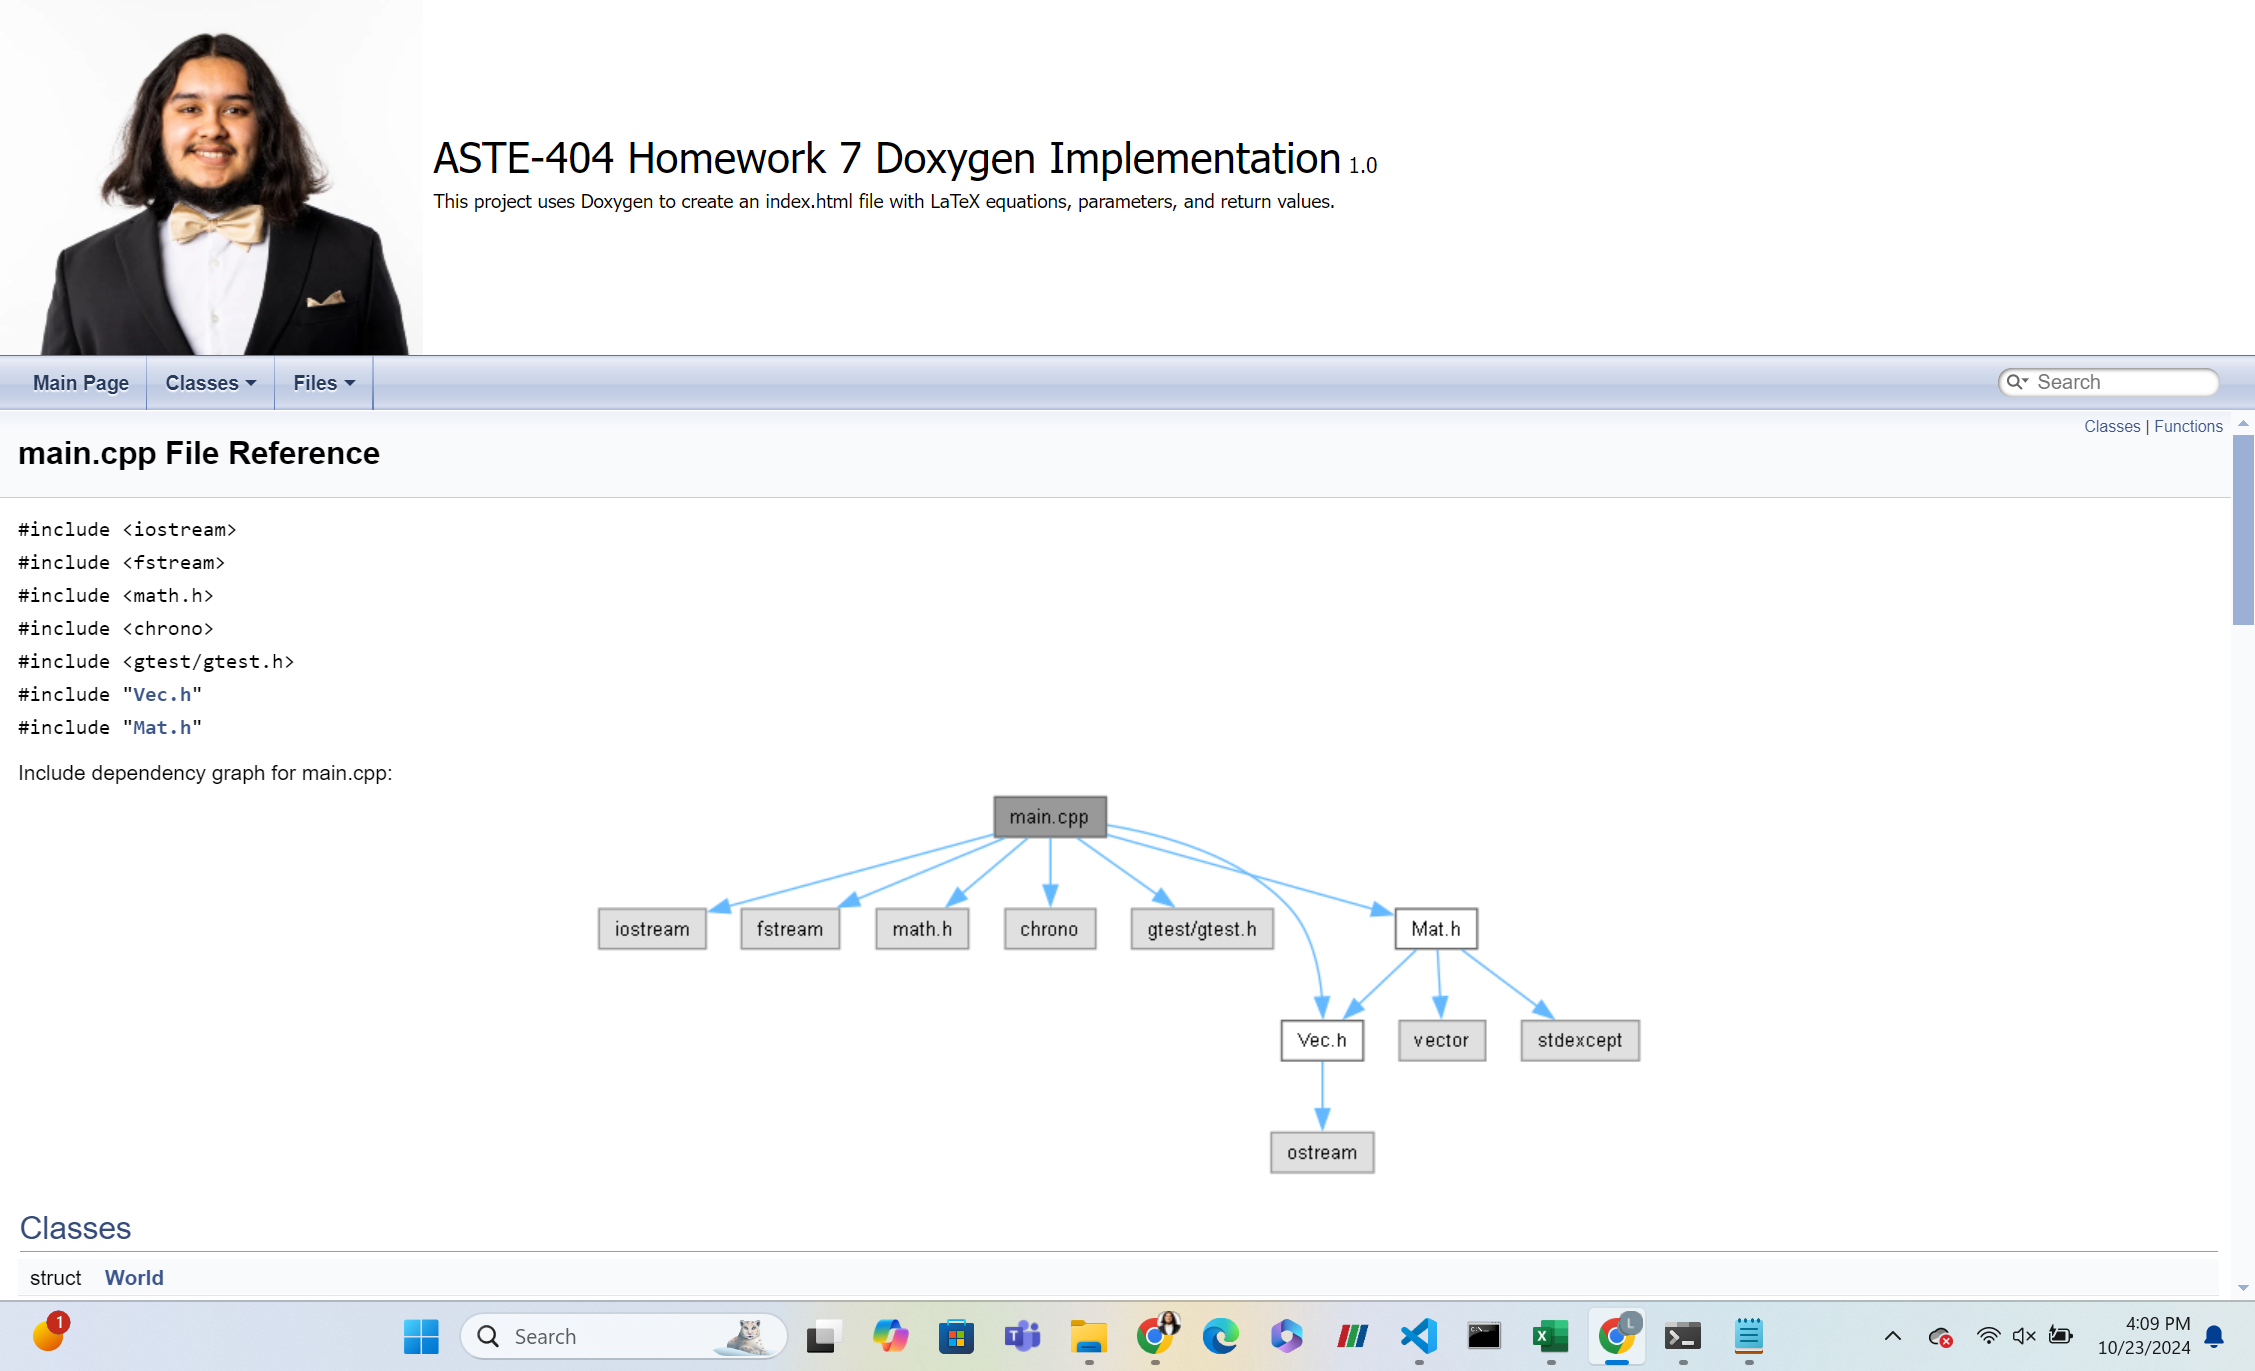
\includegraphics[width=0.8\linewidth]{doxygen.png} % Replace with your screenshot
\caption{Doxygen Documentation Output}
\label{fig:doxygen}
\end{figure}

\section{Part 4: Version Control with Git}
The project was version-controlled using Git and pushed to a GitHub repository. Below are the commands used during the workflow.

\begin{lstlisting}[caption={Git Commands}]
$ git init
$ git add main.cpp vec.h
$ git commit -m "Initial commit"
$ git remote add origin https://github.com/user/repo.git
$ git push -u origin master
\end{lstlisting}

Figure~\ref{fig:github} shows a screenshot of the repository.

\begin{figure}[htbp]
\centering
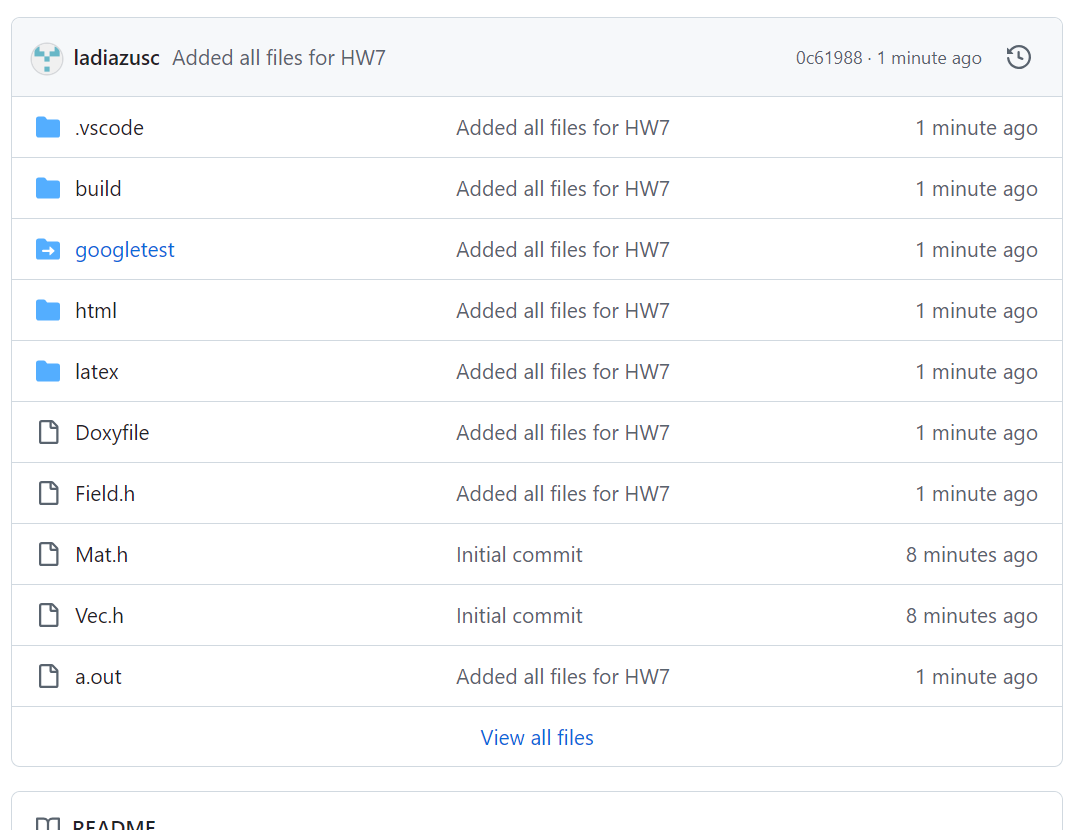
\includegraphics[width=0.8\linewidth]{github.png} % Replace with your screenshot
\caption{GitHub Repository Screenshot}
\label{fig:github}
\end{figure}

\section{Part 5: LaTeX Report Creation}
This document was created using \LaTeX, ensuring professional formatting and precise mathematical typesetting. Figures, code snippets, and hyperlinks were embedded seamlessly.

\section{Conclusion}
This assignment provided practical experience with key software engineering practices. The combination of development, testing, documentation, version control, and reporting promotes the creation of reliable and maintainable software solutions. Several online resources such as \textit{Particle in Cell} and related sites \cite{particleincell, iamlubos, slovakcooking} were valuable in contextualizing the concepts discussed.

\bibliographystyle{IEEEtran}
\bibliography{hw7}

\end{document}
